\begin{prob}
  Sia $ABCDE$ un pentagono convesso t.c. $AB=BC=CD$, $\widehat{EAB}=\widehat{BCD}$ e $\widehat{EDC}=\widehat{CBA}$. Dimostra che la perpendicolare da $E$ a $BC$ e i segmenti $AC$ e $BD$ sono concorrenti.
\end{prob}

\begin{sol}
  Geometria, la mia vecchia nemica. E non un triangolo, nemmeno un quadrato, ma addirittura un pentagono! Devo ammetterlo, quella tesi mi fa venire voglia di baricentriche, ma su quale triangolo? Ogni cosa a suo tempo: prima un bel (si fa per dire...) disegno. Se riesco, vi metto quello fatto a mano. \\

  \begin{center}
    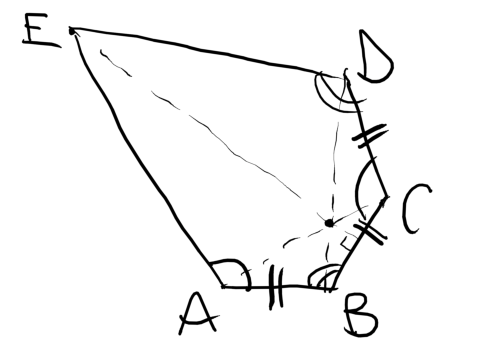
\includegraphics{secs/G1/G1-1.pdf}
  \end{center}

  E adesso, la mia parte preferita: fissarlo finché non mi viene in mente qualche strano elemento geometrico da aggiungere che potrebbe funzionare. Mi è stato detto che ci sono diversi modi per approcciarlo, perciò intanto penso: quale triangolo userei per le baricentriche? Me ne è venuto in mente uno complicato, con un vertice in $E$ e lati $EA, ED, BC$ (quindi prolungando), oppure $EBC$ stesso, ma non mi piacciono i conti che sembrano venir fuori. Anche se quella di prolungare non è una cattiva idea. Devo stare attento, il disegno è (come sempre) viziato: sembrano vere cose che in generale non lo sono, tipo $EA=ED$. Vediamo se riesco a farne uno più generico... Ok, è di nuovo viziato, ma in modo totalmente diverso (ci sono un po' di angoli retti), inoltre sembra essere più accurato ma allo stesso tempo sembra che la tesi sia falsa. Buffo. Ok, no, ricontrollando ho fatto confusione con l'ultima condizione sugli angoli. Guardate il disegno, capirete perché ci sto perdendo tanto tempo - è complicato! Ora va un po' meglio. Ok, vediamo.

  \begin{center}
    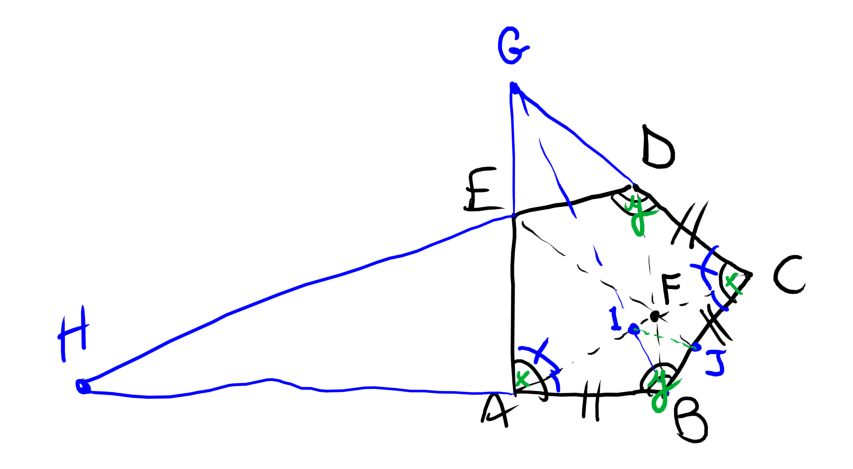
\includegraphics[width=1\textwidth]{secs/G1/G1-2.pdf}
  \end{center}

  Ci sono un po' di triangoli isosceli fatti usando i segmenti $AB, BC, CD$, il che vuol dire angoli uguali, e a noi piacciono gli angoli, ma come gestisco una concorrenza? E ora che ci penso, l'ipotesi sugli angoli farebbe schifo in baricentriche o in qualunque contesto che non sia la geometria sintetica, perciò è da buttare. Oh, giusto! Un classico per gestire le concorrenze è pensarle al contrario: fissiamo due rette, prendiamo la retta che passa per il punto di intersezione e un altro punto obbligato e verifichiamo che coincida con quella che ci manca. In questo caso, procederò così: chiamo $F=AC \cap BD$ e voglio dimostrare che $EF \perp BC$. Leviamo quell'ipotesi dal disegno e mettiamoci $F$. Ah-ah! Ho visto una cosa. Vale la pena tentare. In blu nel disegno trovate le cose che ho aggiunto d'ora in avanti. Da $AB=BC$ otteniamo $\widehat{BAC}=\widehat{BCA}$ che combinato all'ipotesi sugli angoli in $A$ e in $C$ ci dà $\widehat{EAC}=\widehat{DCA}$, perciò se chiamo $G=AE \cap DC$ otterrò che $AGC$ è isoscele di base $AC$. Analogamente, chiamando $H=AB \cap ED$, $BHD$ sarà isoscele di base $BD$. Chissa se queste cose torneranno utili. \\

  Ok, adesso sto provando a vedere un'altra cosa: che angoli ci sono in giro? Per esempio, c'è un modo di calcolare l'angolo $\widehat{AEF}$? Sarebbe perfetto. Vediamo un po'. Così a occhio non mi sembra che ci sia un modo ovvio di trovarlo. Posso impostare delle equazioni per l'angolo $\widehat{AED}$ basate sui poligoni $ABCDE$ e $ACDE$ (o $ABDE$), ma a che servirebbe? E invece il quadrilatero $AFDE$? Promette bene. E c'è anche un'altra cosa che sto considerando: prolungare $AB$ e $DC$ fino alla loro intersezione. Ma non mi ispira più di tanto.

  Ok, sono rimasto silenzioso a fissare la figura per un po', scartando un'idea dopo l'altra, finché non mi sono accorto di una cosa: il quadrilatero $ABCG$ è un deltoide, quindi $AC \perp BG$. Lo stesso per il suo amico $BCDH$. È bello, perché c'è un angolo retto, ma non so come ci possa aiutare. Forse con qualche similitudine! Disegno un paio di rette e guardo i triangoli, se ne trovo due che sembrano somilgiarsi cercherò conferma nell'altro deltoide, in modo da essere sicuro. Ok, fatto. Chiamiamo $I=BG \cap AC$ e $J=EF \cap BC$. Il piano è dimostrare che $ABI$ è simile a $CJF$, in quest'ordine. Si va per angoli. \\

  Meglio passare al verde, così riesco a capire quello che faccio. O forse non avrò neanche bisogno di disegnarli. Facciamo così: chiamiamo $\widehat{EAB}=\widehat{BCD}=x$ e $\widehat{EDC}=\widehat{CBA}=y$. Cominciamo da $\widehat{ABI}=\widehat{ABG}=\pi-x-\widehat{AGB}$. Ora, $\widehat{AGB}=\widehat{AGI}=\pi/2-\widehat{IAG}=\pi/2-(x-(\pi-y)/2)=\pi+(x+y)/2$ (abbiamo sfruttato il fatto che $ABC$ è isoscele), dunque mettendo insieme otteniamo...
  uh, devo aver sbagliato qualche conto, ma sono anche stupido: $\widehat{ABI}=y/2$. Uau. E adesso che guardo la tesi, scopro che in effetti la similitudine che voglio dimostrare è vera (ovvia, a posteriori). E l'uguaglianza per gli angoli in $A$ e in $C$ è gratis. Come faccio allora per calcolare $\widehat{JFC}$? Urge un'altra sessione in cui fisso intensamente il disegno. \\

  Ok, sto seriamente pensando di ritornare all'ipotesi di perpendicolarità, ma voglio comunque sfruttare l'idea di "far fittare la terza retta". Prendo $EF$ e $AC$, quella che deve tornare adesso è $BD$. Intanto abbiamo il quadrilatero $BIFJ$ ciclico (angoli in $I$ e $J$ retti), ma c'è anche un bel po' di angle chasing da fare. Di nuovo a fissare il disegno, stavolta con intenzioni serie. Ok, vediamo: Sappiamo che $\widehat{EDC}=y$ e $\widehat{DCF}=x-(\pi-y)/2$. Sotto queste ipotesi e sfruttando il quadrilatero ciclico, $\widehat{EFC}=\widehat{IFJ}=\pi-\widehat{IBJ}=\pi-y/2$, dunque $\widehat{FED}=2\pi-y-x+(\pi-y)/2-\pi+y/2=\frac{3}{2}\pi-x-y$.
  Non mi piace. O forse sì? Per simmetria dovrebbe essere uguale all'angolo $\widehat{AED}$, perciò oltre che "altezza" quella retta è anche bisettrice... No, sto correndo troppo: stiamo considerando solo il segmento $AC$, altrimenti è come assumere la tesi. Forse ci sono. Ricopio il disegno vuoto per schiarirmi le idee.

  \begin{center}
    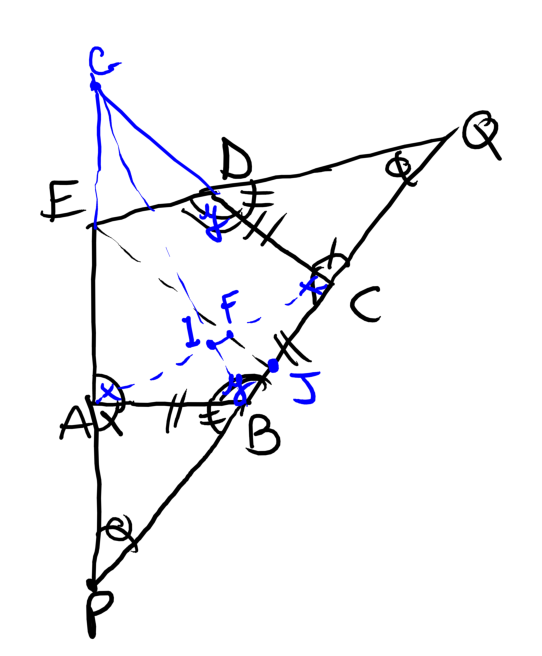
\includegraphics[width=0.54\textwidth]{secs/G1/G1-3.pdf}
  \end{center}

  Siano $P=EA \cap BC$ e $Q=ED \cap BC$. È banale vedere che $EPQ$ è isoscele di base $PQ$, perciò la retta che abbiamo tracciato è sia altezza che bisettrice. Riprendiamo i punti $F$, $G$, $I$ e $J$. Adesso è ovvio che il calcolo di prima era giusto, ma in realtà era ovvio anche prima che fosse davvero la bisettrice. Ehi, è vero, ci sono molti modi per approcciarlo! (E io faccio davvero schifo in sintetica)

  Vediamo se da qui si può concludere, perché tra poco devo andare. Beh, $DB$ si intersecherà da qualche parte con $EJ$, ma se non si intersecasse in $F$ l'angolo formato... no, non funziona. Ok, ho capito cosa mi sta sfuggendo: mi sono scordato che ci sono anche i lati uguali in gioco (almeno, spero sia questo). Ora devo proprio andare, cercherò di non pensarci, magari mi aiuta pure a schiarirmi le idee. \\

  Rieccomi. Sono riuscito a pensarci poco, ho pensato di guardare le lunghezze, ma poi ho scartato subito l'idea, poi mi sono reso conto che forse avevo già visto questo problema (ecco perché una vocina nella mia testa mi diceva "prolunga, prolunga... isoscele, isoscele..."), ma forse vi sarete accorti che non ricordo come si concludeva. Quindi non rimane che dare un'occhiata a quello che ho fatto e vedere se c'è qualcosa che mi sono perso. In effetti, se non mi sbaglio dovrebbe essere possibile dire tutte le cose un minimo rilevanti che ho detto finora senza usare l'ipotesi $BC=CD$; vediamo se c'è qualcosa che si può ottenere da quest'ipotesi che mi sono perso. Ok, qualcosina c'è, ma segue più dall'uguaglianza $AB=CD$ e da ovvie uguaglianze d'angoli: i triangoli $APB$ e $CQD$ sono uguali. Non so se può servire a molto, ma è qualcosa. Non vorrei aver bisogno di un hint per questo problema.

  Non perdiamoci d'animo: torniamo a fissare il disegno. Anzi, proviamo a ragionare così: abbiamo un triangolo isoscele, da cui ai due vertici con angoli uguali tagliamo due triangoli congruenti come quello poc'anzi mensionati. Per questioni di continuità, tutto bello e caruccio, prima o poi si raggiungerà una condizione come quella data dal disegno, e ciò fisserà la posizione di $F$ sulla retta $EJ$. Quindi trovare una lunghezza "neutra" e verificare che effettivamente non cambia per simmetria potrebbe funzionare. Oppure... qualcosa di non neutro ma che dipende sempre della posizione di $F$ e che cambia in modo che l'unico punto che lo possa far funzionare anche dall'altra parte è $F$ stesso (ok, ammetto che questo è un po' troppo contorto). Proviamo.

  Fissiamo $AB=BC=CD=l$. Voglio ad esempio la lunghezza $CQ$. Concentriamoci sul triangolo $CQD$. Gli angoli in $C$ e in $D$ sono rispettivamente $\pi-x$ e $\pi-y$. Di conseguenza, quello in $Q$ è $x+y-\pi$. Per il teorema dei seni, $CQ/\sin{\pi-y}=l/\sin{x+y-\pi} \implies CQ=-l\frac{\sin{y}}{\sin{x+y}}$ (ricordando che il seno può anche essere negativo, ha senso). Con ragionamento analogo, $PB=-l\frac{\sin{x}}{\sin{x+y}}$.
  Perciò $JC=PQ/2-CQ=(PB+l+CQ)/2-CQ=(PB+l-CQ)/2=l\left(1/2+\frac{\sin{y}-\sin{x}}{2\sin{x+y}}\right)$.
  Ricordiamo che, con la costruzione $F=AC \cap EJ$, $\widehat{JCF}=(\pi-y)/2=z$, quindi $JF/JC=\sin{z}/\cos{z} \implies JF=l\left(1/2+\frac{\sin{y}-\sin{x}}{2\sin{x+y}}\right) \cdot \frac{\sin{(\pi-y)/2}}{\cos{(\pi-y)/2}}$, che adesso spero si trasformi in una bellissima espressione simmetrica in $x$ e $y$.
  Intanto trasformiamolo in $l\left(1/2+\frac{\sin{y}-\sin{x}}{2\sin{x+y}}\right) \cdot \frac{\cos{y/2}}{\sin{y/2}}$... Sentite, facciamo una bella cosa: cerco le formule, faccio i conti e vi faccio sapere. Eeed eccomi tornato con buone notizie! Bastava scambiare $x$ e $y$, fare i conti giusti (occhio a non usare bisezione, può essere tricky!) e in effetti l'espressione è simmetrica (viene uguale all'analoga), perciò la lunghezza $JF$ è fissata dagli angoli $x$ e $y$ e dunque è lo stesso punto su $EJ$, sia che si faccia la costruzione intersecando con $AC$, sia con $BD$. Piccola nota: nelle ipotesi c'è quella che il pentagono sia convesso, che aiuta a capire quali seni sono negativi e quali no, così tutti i conti sono validati al cento per cento. \\

  PS: prima o poi mi verrà voglia di aggiungere i disegni.
\end{sol}
